\documentclass[12pt,onecolumn]{article}
\usepackage{amsmath,amssymb}

\usepackage[utf8]{inputenc}
\usepackage{authblk}
\usepackage{setspace}
\usepackage[margin=1in]{geometry}
\usepackage{graphicx}
\graphicspath{{figures/}}
\usepackage{subcaption}
\usepackage{booktabs,tabularx,array}
\usepackage{algorithm}
\usepackage{algpseudocode}
\usepackage{placeins}
\usepackage{lineno}
\usepackage{indentfirst}
\usepackage{tikz}
\usepackage{listings}
\usetikzlibrary{shapes.geometric,arrows.meta,positioning}
\usepackage[hidelinks]{hyperref}
\newcommand{\ESC}{\mathrm{ESC}}
\newcommand{\byte}[1]{\texttt{#1}}



\definecolor{codegreen}{rgb}{0,0.5,0}
\definecolor{codegray}{rgb}{0.5,0.5,0.5}
\definecolor{codepurple}{rgb}{0.58,0,0.82}
\definecolor{codeblue}{rgb}{0,0,0.8}

\lstset{
	language=Python,
	basicstyle=\ttfamily\small,
	keywordstyle=\color{codeblue},
	commentstyle=\color{codegreen},
	stringstyle=\color{codepurple},
	numberstyle=\tiny\color{codegray},
	numbers=left,
	showstringspaces=false,
	breaklines=true,
	frame=single,
	xleftmargin=0pt,
	framexleftmargin=0pt,
	aboveskip=0.5em,
	belowskip=0.5em,
	columns=fullflexible,
	keepspaces=true,
	tabsize=4
}

%opening
\title{Lossless Text Compression Using PPM and Arithmetic Coding}
\author{Zhicheng Li}
\date{}

\onehalfspacing

\begin{document}

\maketitle


% Abstract to be written after the remaining sections.

\section{Overview}
We compress \byte{austen.txt} using order-5 prediction by partial matching
(PPM), update exclusion, tuned probability weights, and 64-bit integer
arithmetic coding. The compressed data and compiled decoder together occupy
23.3358\% of the original size, with exact reconstruction.

\section{Context Modeling and Probability Estimation}
\label{sec:model}

Prediction by partial matching (PPM) provides probability estimates.
An arithmetic coder uses these estimates to produce a compressed bitstream.
PPM estimates the probability of the next symbol using previously observed
symbols as a context. When a longer context cannot predict the next symbol,
the model backs off to a shorter one~\cite{cleary1984}.

\subsection{Context Representation}

Our implementation reads the input file as a sequence of bytes, treating each byte as a symbol from the alphabet $\mathcal{B}=\{0,\ldots,255\}$.
Let $x_t\in\mathcal{B}$ denote the $t$-th input symbol, starting at $t=1$.
The \emph{history} $h$ stores the most recent symbols already processed.
We retain at most $K=5$ symbols, so $|h|=\min(K,t-1)$ before processing $x_t$.
An order-$k$ context $s_k$ consists of the last $k$ symbols of $h$,
where $0\leq k\leq |h|$. The order-0 context is the empty string $\epsilon$.
Thus, $K$ is also the maximum context order.
For each context $s$, a dictionary stores
positive integer counts $c_s(x)$ for the symbols that have been inserted into that
context. Define
\begin{equation}
  \mathcal{A}_s=\{x:c_s(x)>0\}, \qquad U_s=|\mathcal{A}_s|.
\end{equation}
An absent context has an empty table. Contexts are stored as byte-string keys
mapping to symbol-to-count dictionaries.

Both encoder and decoder start with empty dictionaries and empty history.
They construct each prediction table before updating the PPM model with the current
symbol. A \emph{prediction table} lists the available symbols $x$ and their integer
weights $w_s(x)$ for context $s$. These weights are computed from the stored counts and determine the
probability estimates used by the arithmetic coder.
The update rule is described in Section~\ref{sec:model-update}.

\subsection{Context Backoff and Symbol Exclusion}

To construct prediction tables, we first search the available contexts.
The PPM model visits $s_{|h|},s_{|h|-1},\ldots,s_0$ from longest to shortest.

For each new target symbol, initialize an exclusion set $E=\varnothing$.
At the current order-$k$ context $s=s_k$, the available candidates are
\begin{equation}
  \mathcal{V}_s=\mathcal{A}_s\setminus E.
\end{equation}
Here, $\setminus$ denotes set difference: remove all symbols in $E$ from
$\mathcal{A}_s$.
If the target belongs to $\mathcal{V}_s$, encode it using the current context's
prediction table and finish the search.

If $\mathcal{V}_s$ is empty, skip the context without coding an event. This covers
both missing contexts and tables whose symbols have all been excluded.

If $\mathcal{V}_s$ is nonempty but does not contain the target, encode a special
escape event $\ESC$. Each nonempty prediction table contains both
$\mathcal{V}_s$ and $\ESC$. Internally, $\ESC$ is represented by integer 256.
It produces no output symbol. After encoding $\ESC$, set
$E\leftarrow E\cup\mathcal{A}_s$ and continue to the next shorter context.
This backoff mechanism allows the model to encode symbols not yet observed
in the current context~\cite{cleary1984,teahan1995}.

Excluding higher-order predictions from lower-order tables is called
\emph{symbol exclusion}~\cite{teahan1995}. After an escape, these symbols cannot
be the target, so their probability mass can be removed from subsequent symbol
predictions. Symbol exclusion changes the prediction table without modifying
the stored counts.

\begin{figure}[htbp]
\centering
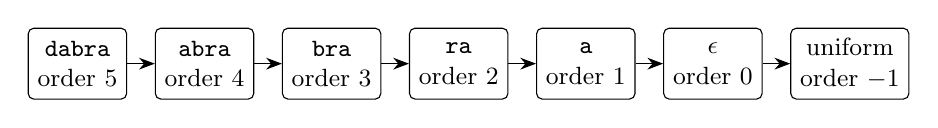
\begin{tikzpicture}[
  context/.style={draw,rounded corners=2pt,minimum width=1.25cm,
    minimum height=0.9cm,align=center,font=\small},
  >={Stealth[length=2mm]},node distance=0.35cm]
  \node[context] (s5) {\byte{dabra}\\order 5};
  \node[context,right=of s5] (s4) {\byte{abra}\\order 4};
  \node[context,right=of s4] (s3) {\byte{bra}\\order 3};
  \node[context,right=of s3] (s2) {\byte{ra}\\order 2};
  \node[context,right=of s2] (s1) {\byte{a}\\order 1};
  \node[context,right=of s1] (s0) {$\epsilon$\\order 0};
  \node[context,right=of s0] (sm) {uniform\\order $-1$};
  \foreach \a/\b in {s5/s4,s4/s3,s3/s2,s2/s1,s1/s0,s0/sm}
    \draw[->] (\a) -- (\b);
\end{tikzpicture}
\caption{Search order for history \byte{dabra}. Follow an arrow after an escape
or an empty candidate set; stop when the target symbol is encoded. Each shorter
nonnegative-order context removes the preceding context's first symbol.}
\label{fig:backoff}
\end{figure}

If all nonnegative orders fail to find the target, use the order-$-1$ table. It assigns integer
weight 1 to every symbol in $\mathcal{B}\setminus E$, with no escape event:
\begin{equation}
  P_{-1}(x\mid E)=\frac{1}{256-|E|},
  \qquad x\in\mathcal{B}\setminus E.
\end{equation}
Thus a previously unseen symbol can always be encoded. In particular, the first
input symbol is encoded using the uniform distribution over all 256 symbols.

\subsection{Model Update}
\label{sec:model-update}

After the arithmetic coder encodes or decodes the input symbol $x_t$,
visit the contexts from longest to shortest.
If a context $s$ does not contain $x_t$, set $c_s(x_t)=1$ and continue
to the next shorter context. Create an empty table first if the context is
missing. At the first context that already contains $x_t$, increment its count
by 1 and stop. All shorter contexts remain unchanged.

This rule is called \emph{update exclusion}~\cite{teahan1995}. It determines
which stored counts change, whereas symbol exclusion determines which symbols
are available during prediction. Consequently, the stored counts need not equal
substring occurrence counts.

Finally, append $x_t$ to the history and retain only its last $K$ symbols.
Both counts and history are updated once per input symbol. No updates occur
between successive escapes for the same symbol.

\subsection{Tuned Integer Weights}

Before symbol exclusion, standard PPM-D assigns integer weights $2c_s(x)-1$
to known symbols and $U_s$ to escape~\cite{howard1992}. Inspired by this
estimator, we instead use:
\begin{equation}
  w_s(x)=200c_s(x)\quad(x\in\mathcal{V}_s),
  \qquad w_s(\ESC)=86U_s.
  \label{eq:weights}
\end{equation}
The constants 200 and 86 were chosen experimentally for this implementation;
their selection is evaluated in Section~\ref{sec:experiments}.

For each nonempty candidate set, the normalizing total and probabilities are
\begin{align}
  T_s(E)&=200\sum_{x\in\mathcal{V}_s}c_s(x)+86U_s,\\
  P_s(x\mid E)&=\frac{200c_s(x)}{T_s(E)},
  &P_s(\ESC\mid E)&=\frac{86U_s}{T_s(E)}.
  \label{eq:probabilities}
\end{align}
Importantly, $U_s$ counts \emph{all} distinct symbols stored in the context,
including excluded ones. Only the symbol term in $T_s(E)$ uses the reduced
candidate set. The implementation does not replace $U_s$ with
$|\mathcal{V}_s|$.

Available symbols are ordered by increasing numeric value, followed by $\ESC$;
the order-$-1$ table uses the same symbol ordering. The arithmetic coder uses the
weights and cumulative sums directly. The decoder reconstructs the same tables
and updates only after recovering a symbol, so frequency tables are not transmitted.

\subsection{Worked Example}

Consider encoding a space after \byte{abracadabra}. Table~\ref{tab:example} shows
the state produced by the actual order-5 implementation with update exclusion.
Symbols are displayed as ASCII characters. The history is \byte{dabra}, giving the search order
in Figure~\ref{fig:backoff}.

\begin{table}[htbp]
\centering
\begingroup
\setstretch{1}
\small
\setlength{\tabcolsep}{4pt}
\renewcommand{\arraystretch}{1.35}
\begin{tabularx}{\textwidth}{@{}c l >{\raggedright\arraybackslash}X
  >{\raggedright\arraybackslash}p{2.05cm}
  >{\raggedright\arraybackslash}p{3.55cm} l@{}}
\toprule
Order & Context & Stored counts & Excluded $E$ & Available weights & Action\\
\midrule
5 & \byte{dabra} & none & $\varnothing$ & none & skip\\
4 & \byte{abra} & $c:1$ & $\varnothing$ & $c:200,\ \ESC:86$ & $\ESC$\\
3 & \byte{bra} & $c:1$ & $\{c\}$ & none & skip\\
2 & \byte{ra} & $c:1$ & $\{c\}$ & none & skip\\
1 & \byte{a} & $b:2,\ c:1,\ d:1$ & $\{c\}$ &
  $b:400,\ d:200,$\newline $\ESC:258$ & $\ESC$\\
0 & $\epsilon$ & $a:4,\ b:1,\ c:1,$\newline $d:1,\ r:1$ & $\{b,c,d\}$ &
  $a:800,\ r:200,$\newline $\ESC:430$ & $\ESC$\\
$-1$ & default & not stored & $\{a,b,c,d,r\}$ &
  251 remaining symbols, each with weight 1 & space\\
\bottomrule
\end{tabularx}
\endgroup
\caption{Model trace for a space after \byte{abracadabra}. Exclusion sets are
shown on entry to each row; skipped contexts produce no coding event.}
\label{tab:example}
\end{table}

\begin{samepage}
Order 5 is missing. The order-4 escape excludes \byte{c}, leaving no candidates
at orders 3 and 2. At order 1, the remaining symbol weights are 400 and 200,
but the escape weight is $86\times3=258$: the excluded \byte{c} still contributes
to $U_s$. The next escape also excludes \byte{b} and \byte{d}. Order 0 retains
only \byte{a} and \byte{r}, while its escape weight uses all five stored symbols.
\end{samepage}

\begin{samepage}
The event sequence supplied to the arithmetic coder is therefore
\begin{equation}
  \ESC_{4},\quad \ESC_{1},\quad \ESC_{0},\quad
  \text{space}_{-1},
\end{equation}
where subscripts indicate context order. Its model probability, before integer
interval rounding, is
\begin{equation}
  P(\text{space}\mid\byte{abracadabra})
  =\frac{86}{286}\,\frac{258}{858}\,\frac{430}{1430}\,
    \frac{1}{251}.
\end{equation}
\end{samepage}
Only after this complete sequence do encoder and decoder update their counts
and history with the space. This illustrates how a single input symbol may
require several coding events while still producing exactly one output symbol.
\FloatBarrier

\section{Integer Arithmetic Coding}
\label{sec:arithmetic}

The PPM model supplies a prediction table for each coding event.
The arithmetic coder uses its integer weights to narrow a numeric interval.
As the interval narrows, the coder outputs bits that identify the selected
interval. We use the integer coding framework described by Witten, Neal, and
Cleary~\cite{witten1987} and Howard and Vitter~\cite{howard1992}.
The rules below specify our implementation, including its 64-bit state and
bitstream termination.

\subsection{Prediction Tables and Coding State}

Let $e_0,\ldots,e_{m-1}$ be the $m$ entries of the current prediction table,
in encoding order. Each entry is an available input symbol or $\ESC$.
Let $w_j$ denote the integer weight of entry $e_j$.
For a nonnegative-order context $s$, this is $w_s(e_j)$ from
Equation~\eqref{eq:weights}. At order $-1$, every entry has weight 1.
Define the cumulative weights and total weight as
\begin{equation}
  C_0=0,\qquad C_j=\sum_{i=0}^{j-1}w_i\quad(1\leq j\leq m),
  \qquad T=C_m.
  \label{eq:cumulative}
\end{equation}
Thus, entry $e_j$ has cumulative range $[C_j,C_{j+1})$ and probability
estimate $w_j/T$. The ordering is the one defined in the preceding section:
increasing symbol values, followed by $\ESC$ when present.

The coder maintains an integer interval $[L,H]$, including both endpoints.
We define
\begin{equation}
  F=2^{64},\qquad M=F/2,\qquad Q=F/4,
  \qquad L=0,\quad H=F-1.
\end{equation}
Here, $F$ is the size of the full range, $M$ its midpoint, and $Q$ one quarter
of its size. The interval is initialized once per file. It is carried across
all coding events, including escapes and changes of context.
Python integers allow intermediate widths and products to exceed 64 bits
without overflow. All divisions below use integer arithmetic.

\subsection{Interval Update}

To encode entry $e_j$, first compute the current interval width
$R=H-L+1$. Then select its subinterval:
\begin{align}
  L'&=L+\left\lfloor\frac{R C_j}{T}\right\rfloor,\label{eq:ac-low}\\
  H'&=L+\left\lfloor\frac{R C_{j+1}}{T}\right\rfloor-1.
  \label{eq:ac-high}
\end{align}
Both expressions use the old value of $L$. Replace $(L,H)$ with $(L',H')$
only after computing both endpoints. The floor operation $\lfloor z\rfloor$
rounds $z$ down to an integer. Larger weights receive wider subintervals,
up to integer rounding.

\subsection{Renormalization and Bit Output}

After an interval update, the coder checks the three cases in
Table~\ref{tab:renormalization}.
This step is called \emph{renormalization}. It lets the coder output known
bits while keeping the interval within the fixed range.

Some bits must wait until a preceding bit is known.
Let $p$ count these \emph{pending bits}, with $p=0$ initially.
Define $\operatorname{emit}(b)$ for a bit $b\in\{0,1\}$ as follows:
output $b$, then output $p$ copies of $1-b$, and reset $p$ to zero.
For example, if $p=0$, then $\operatorname{emit}(0)$ outputs \byte{0}; if $p=2$, then $\operatorname{emit}(0)$ outputs \byte{011}.

\begin{table}[htbp]
\centering
\begingroup
\setstretch{1}
\small
\renewcommand{\arraystretch}{1.4}
\begin{tabularx}{\textwidth}{@{}l l c X@{}}
\toprule
Case & Interval condition & Offset $\delta$ & Encoder action\\
\midrule
E1 & $H<M$ & $0$ & $\operatorname{emit}(0)$\\
E2 & $L\geq M$ & $M$ & $\operatorname{emit}(1)$\\
E3 & $Q\leq L<M\leq H<3Q$ & $Q$ & Increase $p$ by 1; output no bit yet\\
\bottomrule
\end{tabularx}
\endgroup
\caption{Renormalization rules. Subtract the offset $\delta$ from each endpoint
before shifting left by one bit. Apply the rules repeatedly after every coding event.}
\label{tab:renormalization}
\end{table}



For the selected case, perform its encoder action.
Let $z\ll1$ denote a one-bit left shift of a nonnegative integer $z$.
Update the endpoints as follows:
\begin{equation}
  L\leftarrow (L-\delta)\ll1,\qquad
  H\leftarrow \bigl((H-\delta)\ll1\bigr)+1.
  \label{eq:renormalize}
\end{equation}
The left shift appends a 0 to $L$. For $H$, the additional $+1$ appends a 1
instead, preserving the inclusive upper endpoint.
Check the conditions again using the new endpoints.
Stop renormalizing when none applies, then process the next coding event.
In E1 and E2, the interval determines the next output bit.
In E3, that bit is still uncertain. Each E3 step records a following bit
that will be the complement of the eventual output bit.
The pending count is retained across coding events until an
$\operatorname{emit}$ operation resolves it.

\subsection{Final Bit Emission}
\label{sec:ac-finalization}

After all input symbols have been encoded, the encoder must finish the
remaining interval. For nonempty input, first increase $p$ by 1.
Then apply
\begin{equation}
  \begin{cases}
    \operatorname{emit}(0),&L<Q,\\
    \operatorname{emit}(1),&L\geq Q.
  \end{cases}
  \label{eq:ac-finalize}
\end{equation}
This final emission selects a bit prefix for the remaining interval and
resolves the pending bits.

\subsection{Arithmetic Decoding}
\label{sec:ac-decoding}

The arithmetic decoder starts with the same interval $[0,F-1]$.
It also maintains a \emph{code value} $V$. Initialize $V=0$, then read the
first 64 bits of the payload in order. For each bit $b$, set
$V\leftarrow (V\ll1)+b$. Payload bit order and zero-padding are specified
in Section~\ref{sec:bit-packing}.

For the current prediction table, compute its cumulative weights and
$R=H-L+1$. Map $V$ into the cumulative-weight range using
\begin{equation}
  u=\left\lfloor
    \frac{(V-L+1)T-1}{R}
  \right\rfloor.
  \label{eq:ac-decode}
\end{equation}
Choose the unique entry $e_j$ satisfying $C_j\leq u<C_{j+1}$.
Use that entry to update the interval with
Equations~\eqref{eq:ac-low}--\eqref{eq:ac-high}.
The decoder then applies the same renormalization cases as the encoder.
For each case, use its offset $\delta$ in Equation~\eqref{eq:renormalize}
and update the code value as
\begin{equation}
  V\leftarrow \bigl((V-\delta)\ll1\bigr)+b,
\end{equation}
where $b$ is the next payload bit. Repeat until no case applies.
The decoder reads bits rather than emitting them; it does not maintain a
pending-bit count.
The recovered event $e_j$ is returned to the PPM model.
The file-level loop that requests these events is described next.
\FloatBarrier

\section{Compressed File Format and Reconstruction}
\label{sec:file-format}
\label{sec:bit-packing}

The file contains the original byte count $N$ followed by an arithmetic-coded
payload. Both encoder and decoder use $K=5$, the same 64-bit arithmetic
state and weights, and initially empty context statistics.

\begin{table}[htbp]
\centering
\begingroup
\setstretch{1}
\small
\renewcommand{\arraystretch}{1.4}
\begin{tabularx}{\textwidth}{@{}l l X@{}}
\toprule
Byte offset & Field & Representation\\
\midrule
0--3 & Original length $N$ & Unsigned 32-bit integer, little-endian\\
4 onward & Arithmetic-coded payload & Bits packed most significant bit first\\
\bottomrule
\end{tabularx}
\endgroup
\caption{Compressed file layout. The header occupies exactly four bytes.
The payload size depends on the input and the model's predictions.}
\label{tab:file-layout}
\end{table}

Payload bits are packed most significant bit first, with zeros filling any
unused low bits of the final byte. The decoder reads from byte offset 4
in the same order; requests beyond the payload return zero, including when
initializing the 64-bit code value. It stops after recovering exactly $N$
bytes; escapes produce no output and do not advance this count. Empty input
is represented by four zero header bytes and no payload. No end-of-file
event is encoded.

For each input byte, the encoder processes the backoff tables until the
byte is encoded, then updates the model once. After the last byte, it emits
the final bits as specified in Section~\ref{sec:ac-finalization} and writes
the header and packed payload to \byte{compressed}. The decoder follows
the same table sequence until a non-escape symbol is recovered, writes that
byte to \byte{out.txt}, and updates the model. Both sides retain their
arithmetic state across all events and use binary file input and output.
\FloatBarrier

\section{Experiments and Results}
\label{sec:experiments}

\subsection{Experimental Setup}

All methods use the same \byte{austen.txt} input of $N=2{,}664{,}245$ bytes.
Let $C$ denote the complete compressed-file size and $D$ the compiled-decoder
size. The evaluation metric is
\begin{equation}
  R_{\mathrm{total}}=\frac{C+D}{N}\times100\%.
  \label{eq:total-ratio}
\end{equation}
All decoders were minified with python-minifier 3.2.0 and compiled at
optimization level 0 with the embedded filename \byte{decompress.py}.
Measurements used an Apple M3 running macOS 26.7.1 and Python 3.12.4;
reported times are median user CPU times from three runs of the compiled
decoder, measured with \byte{/usr/bin/time -p}.
All 20 configurations reproduced the input byte for byte in all three runs.
Parameter tuning uses this same input, so the selected settings are
specific to this file.

\subsection{Parameter Selection}

Table~\ref{tab:order-selection} varies the context order while fixing the
tuned weights, update exclusion, arithmetic coder, and four-byte header.
Order 5 produces the smallest file among the tested orders, saving
23,411 bytes over order 4 and 3,648 bytes over order 6.

\begin{table}[htbp]
\centering
\begingroup
\setstretch{1}
\small
\renewcommand{\arraystretch}{1.35}
\begin{tabular}{@{}c r@{}}
\toprule
Maximum order $K$ & Compressed size $C$ (bytes)\\
\midrule
4 & 640,200 \\
5 (selected) & 616,789 \\
6 & 620,437 \\
\bottomrule
\end{tabular}
\endgroup
\caption{Context-order comparison. All three decoders occupy 4,934 bytes.}
\label{tab:order-selection}
\end{table}

Figure~\ref{fig:escape-weight} compares nine escape factors between 80 and 110,
with the symbol factor fixed at 200 and $K=5$.
The selected factor $\beta=86$ gives the smallest
file, but saves only one byte over 87. Relative to the untuned weights
$2c_s(x)$ and $U_s$, tuning saves 422 compressed bytes under the same header;
this is a small additional improvement.

\begin{figure}[htbp]
\centering
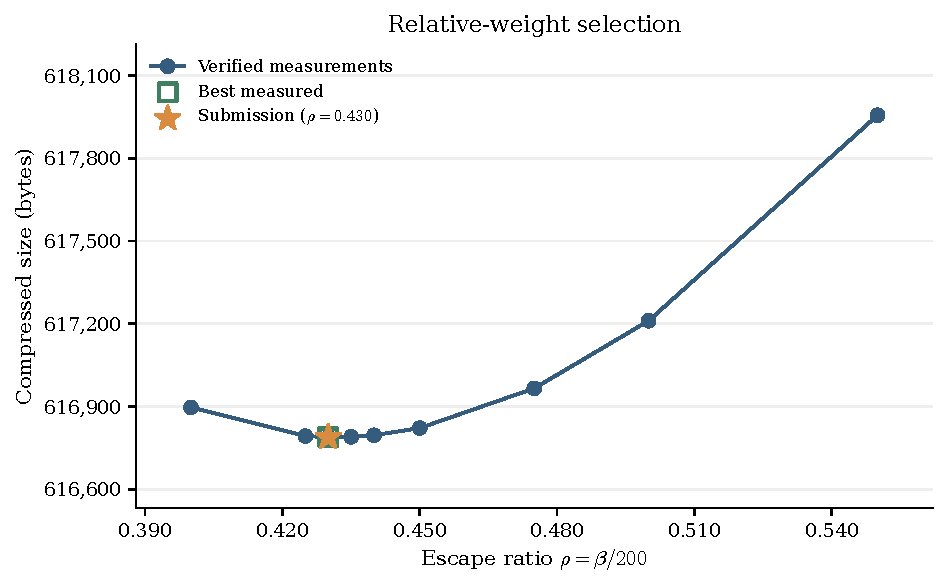
\includegraphics[width=0.72\textwidth]{escape_weight.pdf}
\caption{Escape-weight tuning at $K=5$, with $\rho=\beta/200$.
The smallest file occurs at $\beta=86$ ($\rho=0.43$).}
\label{fig:escape-weight}
\end{figure}
\FloatBarrier

\subsection{Comparison with Other Compression Algorithms}

The baselines are two-byte Huffman coding~\cite{huffman1952}, static
arithmetic coding~\cite{witten1987}, LZ78~\cite{ziv1978}, and LZW~\cite{welch1984}.
Their compressed sizes include the Huffman tree, static frequency table,
or dictionary-code headers as applicable. LZ78 and LZW use fixed whole-byte
index widths.

\begin{table}[htbp]
\centering
\begingroup
\setstretch{1}
\small
\setlength{\tabcolsep}{4pt}
\renewcommand{\arraystretch}{1.4}
\begin{tabularx}{\textwidth}{@{}X r r r r@{}}
\toprule
Method & \shortstack{Compressed\\bytes $C$} &
  \shortstack{Decoder\\bytes $D$} & $R_{\mathrm{total}}$ &
  \shortstack{Decode CPU\\time (s)}\\
\midrule
Huffman (two-byte groups) & 1,308,812 & 3,300 & 49.2489\% & 0.49 \\
Context-free arithmetic coding$^{*}$ & 1,444,892 & 2,844 & 54.3394\% & 4.28 \\
LZ78 & 1,475,432 & 1,414 & 55.4321\% & 0.10 \\
LZW & 1,247,197 & 1,578 & 46.8716\% & 0.15 \\
Final tuned PPM + UE + arithmetic & 616,789 & 4,934 & 23.3358\% & 7.73 \\
\bottomrule
\end{tabularx}
\endgroup
\caption{Size and decoding user CPU time (median of three runs). The starred
baseline imports \byte{bisect}, which is not permitted for submission.}
\label{tab:algorithm-comparison}
\end{table}

The final method has the smallest total size among these implementations,
using 50.21\% less storage than LZW, the next smallest baseline.
Its median decoding time is 7.73 seconds (range 7.62--7.91 seconds), slower
than all four baselines. These results apply to this input and the tested
implementations. The final decoder imports no modules; runtime validation
on the required ECE Linux host remains separate from these local measurements.
\FloatBarrier

\section{CONCLUSIONS}

On the project input, the selected order-5 PPM model with update exclusion,
weights $200c_s(x)$ and $86U_s$, and 64-bit integer arithmetic coding produces
a 616,789-byte compressed file and a 4,934-byte compiled decoder. Their
combined size is 621,723 bytes, or 23.3358\% of the original. All three
measured decoding runs reconstruct the input exactly, with a median local
user CPU time of 7.73 seconds. The parameter comparisons support the
selected settings among the tested candidates. The final method
uses the least storage among the tested implementations but decodes more
slowly. These conclusions are specific to this input and local environment;
ECE Linux runtime validation remains separate.

\section{Acknowledgments}

The main algorithmic ideas come from prior work: PPM and context backoff
from Cleary and Witten~\cite{cleary1984}, probability estimation and exclusion
rules from Teahan~\cite{teahan1995}, and integer arithmetic coding from
Witten et al.~\cite{witten1987} and Howard and Vitter~\cite{howard1992}.
Before developing the final method, I explored Huffman coding, arithmetic
coding, LZ78, and LZW using code obtained from online sources or generated
with AI assistance. The Huffman implementation was adapted from a
GeeksforGeeks example~\cite{gfg-code}; the LZ78 and LZW implementations were
adapted from Yousef Javaherian's LZW example on Stack Overflow~\cite{so-code}.
I reviewed and modified these implementations, including testing two-byte
symbols to improve Huffman compression.

After these trials, I asked AI for a suitable approach for this text.
It recommended PPM with arithmetic coding and generated an initial PPM
extension to the existing arithmetic coder, substantially improving
compression. I then refined parameters and implementation structure using
AI suggestions, online references, and my own reasoning, obtaining smaller
additional gains. My contributions included reviewing the code, evaluating
the alternatives, and refining the design; AI assisted with code generation
and revision, as well as drafting and editing parts of this report.

\begin{singlespace}
\begin{thebibliography}{9}

\bibitem{cleary1984}
J.~G. Cleary and I.~H. Witten,
``Data compression using adaptive coding and partial string matching,''
\emph{IEEE Transactions on Communications}, vol.~32, no.~4,
pp.~396--402, 1984.
\href{https://doi.org/10.1109/TCOM.1984.1096090}{doi:10.1109/TCOM.1984.1096090}.

\bibitem{teahan1995}
W.~J. Teahan,
``Probability estimation for PPM,''
in \emph{Proceedings of the New Zealand Computer Science Research Students
Conference}, University of Waikato, Hamilton, New Zealand,
pp.~267--274, 1995.
\href{https://cotty.16x16.com/compress/peppm.htm}{Online text}.

\bibitem{howard1992}
P.~G. Howard and J.~S. Vitter,
``Practical implementations of arithmetic coding,''
in \emph{Image and Text Compression}, J.~A. Storer, Ed.
Kluwer Academic Publishers, 1992, pp.~85--112.
\href{https://www.ittc.ku.edu/~jsv/Papers/HoV92.actech.pdf}{Technical report version}.

\bibitem{witten1987}
I.~H. Witten, R.~M. Neal, and J.~G. Cleary,
``Arithmetic coding for data compression,''
\emph{Communications of the ACM}, vol.~30, no.~6, pp.~520--540, 1987.
\href{https://doi.org/10.1145/214762.214771}{doi:10.1145/214762.214771}.

\bibitem{huffman1952}
D.~A. Huffman,
``A method for the construction of minimum-redundancy codes,''
\emph{Proceedings of the IRE}, vol.~40, no.~9, pp.~1098--1101, 1952.
\href{https://doi.org/10.1109/JRPROC.1952.273898}{doi:10.1109/JRPROC.1952.273898}.

\bibitem{ziv1978}
J. Ziv and A. Lempel,
``Compression of individual sequences via variable-rate coding,''
\emph{IEEE Transactions on Information Theory}, vol.~24, no.~5,
pp.~530--536, 1978.
\href{https://doi.org/10.1109/TIT.1978.1055934}{doi:10.1109/TIT.1978.1055934}.

\bibitem{welch1984}
T.~A. Welch,
``A technique for high-performance data compression,''
\emph{Computer}, vol.~17, no.~6, pp.~8--19, 1984.
\href{https://doi.org/10.1109/MC.1984.1659158}{doi:10.1109/MC.1984.1659158}.

\bibitem{gfg-code}
GeeksforGeeks, ``Huffman Coding in Python,'' online code example.
\href{https://www.geeksforgeeks.org/dsa/huffman-coding-in-python/}{Source},
accessed October 20, 2026.

\bibitem{so-code}
Y.~Javaherian, Python LZW code example, Stack Overflow answer.
\href{https://stackoverflow.com/a/77656917}{Source},
accessed October 20, 2026.

\end{thebibliography}
\end{singlespace}

\appendix
\section{Unminified Decoder Source}

The submitted Python decoder is automatically minified using
\byte{python-minifier} to reduce its source size, which also reduces the
compiled \byte{.pyc} size in our implementation. For readability, this
appendix presents the original, unminified decoder source.

% Insert the original, unminified decoder source below.

\begin{lstlisting}[language=Python, caption={My First Python Listing}]
STATE_BITS = 64
FULL_RANGE = 1 << STATE_BITS
HALF = FULL_RANGE >> 1
QUARTER = HALF >> 1
MASK = FULL_RANGE - 1
ESCAPE = 256

class PPMModel:
    def __init__(self):
        self.history = b""
        self.contexts = {}

    def distributions(self):
        # Start with the longest context, shortening it after each ESCAPE.
        excluded = set()
        for order in range(len(self.history), -1, -1):
            context = self.history[-order:] if order else b""
            counts_table = self.contexts.get(context, {})
            frequencies = [(symbol, 200 * count) for symbol, count in sorted(counts_table.items())
                           if symbol not in excluded]
            if not frequencies:
                continue
            # Match the encoder's 200 * count weights; ESCAPE gets 86 per
            # distinct symbol, including those removed by exclusion.
            frequencies.append((ESCAPE, 86 * len(counts_table)))
            yield frequencies
            excluded.update(counts_table)

        # Order -1: all remaining byte values have equal probability.
        yield [(symbol, 1) for symbol in range(256) if symbol not in excluded]

    def update(self, symbol):
        # Insert into escaped contexts, increment the first predicting one,
        # then exclude every lower order from this update.
        for order in range(len(self.history), -1, -1):
            context = self.history[-order:] if order else b""
            counts_table = self.contexts.setdefault(context, {})
            if symbol in counts_table:
                counts_table[symbol] += 1
                break
            counts_table[symbol] = 1
        self.history = (self.history + bytes([symbol]))[-5:]


def arithmetic_decompress(data):
    original_size = int.from_bytes(data[:4], "little")

    bit_position = 4 * 8
    bit_limit = len(data) * 8

    def read_bit():
        nonlocal bit_position
        if bit_position < bit_limit:
            bit = (data[bit_position // 8] >> (7 - bit_position % 8)) & 1
        else:
            bit = 0
        bit_position += 1
        return bit

    low = 0
    high = MASK
    value = 0
    for _ in range(STATE_BITS):
        value = (value << 1) | read_bit()

    def decode_symbol(frequencies):
        nonlocal low, high, value
        total = sum(count for _, count in frequencies)
        width = high - low + 1
        scaled = ((value - low + 1) * total - 1) // width
        lower = 0
        for symbol, count in frequencies:
            if scaled < lower + count:
                break
            lower += count

        high = low + width * (lower + count) // total - 1
        low = low + width * lower // total
        while True:
            if (high & HALF) == 0:
                pass
            elif (low & HALF) != 0:
                low -= HALF
                high -= HALF
                value -= HALF
            elif (low & QUARTER) != 0 and (high & QUARTER) == 0:
                low -= QUARTER
                high -= QUARTER
                value -= QUARTER
            else:
                break
            low <<= 1
            high = (high << 1) | 1
            value = (value << 1) | read_bit()
        return symbol

    model = PPMModel()
    output = bytearray()
    for _ in range(original_size):
        for frequencies in model.distributions():
            symbol = decode_symbol(frequencies)
            if symbol != ESCAPE:
                break
        output.append(symbol)
        model.update(symbol)
    return output


with open("compressed", "rb") as fin, open("out.txt", "wb") as fout:
    fout.write(arithmetic_decompress(fin.read()))
\end{lstlisting}

\end{document}
